\documentclass{article}
\usepackage[utf8]{inputenc}
\usepackage{longtable}
\usepackage{pgfplots}
\usepackage{amsfonts}
\usepackage{graphicx}
\usepackage{fullpage}
\usepackage{amsmath}
\usepackage{amssymb}
\usepackage{natbib}


\pgfplotsset{compat=newest}
\title{Linear Regression}
\author{TDung}
\date{------------------------------------------}

\begin{document}
\tableofcontents

\maketitle
\section{Introduction}
    \begin{center}
        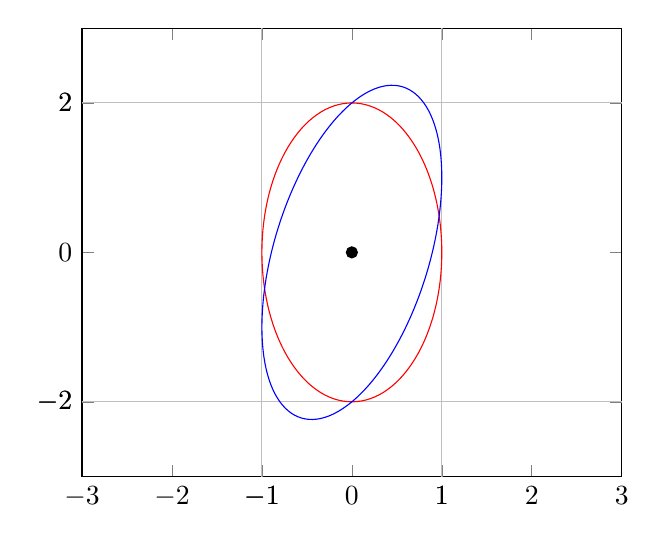
\begin{tikzpicture}
            \begin{axis}[
            	xmin=-3,   xmax=3,
            	ymin=-3,   ymax=3,
            	extra x ticks={-1,1},
            	extra y ticks={-2,2},
            	extra tick style={grid=major},
            ]
            	\draw[red] \pgfextra{
            	  \pgfpathellipse{\pgfplotspointaxisxy{0}{0}}
            		{\pgfplotspointaxisdirectionxy{1}{0}}
            		{\pgfplotspointaxisdirectionxy{0}{2}}
            	};
            	\draw[blue] \pgfextra{
            	  \pgfpathellipse{\pgfplotspointaxisxy{0}{0}}
            		{\pgfplotspointaxisdirectionxy{1}{1}}
            		{\pgfplotspointaxisdirectionxy{0}{2}}
            	};
            	\addplot [only marks,mark=*] coordinates { (0,0) };
            \end{axis}  
        \end{tikzpicture}
    \end{center}
	Linear regression is used to predict value of a variable based on the value of another one. The variable using to predict the other one is called \textit{Independent variable} (or sometimes, it might be called \textit{predictor variable}).The predicted variable is called \textit{dependent variable} (or sometimes, it might be called \textit{the outcome variable}).
	
    For example, you can use linear regression to predict the population of a country based on the population of previous years or maybe you can predict a person's height depends on their weight...
    
    In case we have more than one independent variable, we have to use multiple regression.
    
\section{Ordinary Least Squares Estimation} 
	\textit{Simple linear regression} model includes the \textit{mean function}(1) and the \textit{variance function}(2). 
	\begin{align}
            &E = (Y|X=x) = \beta _{0} + \beta _{1} x \\
            &Var(Y|X=x) = \sigma ^ {2}
    \end{align}
    In this line, Y is the output variable we want to predict, X is the input variable we know, $\beta_{0}$ and $\beta_{1}$ are the coefficients we need to estimate that can move the line around.
    
    The parameters in the \textit{mean function} (1) are the intercept ${\beta _{0}}$ and the slope ${\beta_{1}}$. The intercept is the value of ${E(Y |X = x)}$ when x equals to zero (\textit{in machine learning, it is called the bias, because it is added to offset all predictions}) and the slope is defined by change in ${E(Y |X = x)}$ for a unit change in X. The parameters are usually unknown and must be estimated by using data. By changing the parameters, we can get all possible straight lines.
    
    The \textit{variance function} (2) is assumed to be constant, with a positive value ${\sigma ^ {2}}$ that is usually unknown. When ${\sigma ^ {2} > 0}$, the observed value of the ${i^{th}}$ response ${y_{i}}$ will typically not equal to its expected value ${E(Y|X=x_{i})}$. 
    \begin{center}
        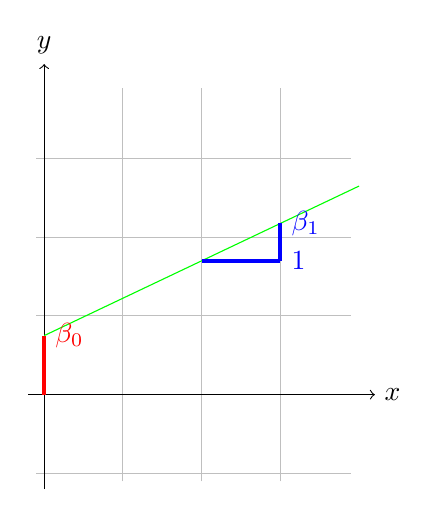
\begin{tikzpicture}[domain=0:4]
            \draw[thin,color=gray!50] (-0.1,-1.1) grid (3.9,3.9);
            \draw[->] (-0.2,0) -- (4.2,0) node[right] {$x$};
            \draw[->] (0,-1.2) -- (0,4.2) node[above] {$y$};
            \draw[domain=0:4, color=green] plot (\x,0.475*\x + 0.75) node[right] {${}$};
            \draw (0,0)--(0,0.75);
            \draw [line width=1.5, red] (0,0)--(0,0.75) node[right] {${\beta _{0}}$}; 
            \draw [line width=1.5, blue] (2,1.7)--(3,1.7) node[right] {${1}$}; 
            \draw [line width=1.5, blue] (3,1.7)--(3,2.175) node[right] {${\beta _{1}}$}; 
        \end{tikzpicture}
        
        \textit{Equation of a straight line ${E(Y|X=x)=\beta _{0} + \beta _{1} x}$} 
    \end{center}
    
    There are many methods for obtaining estimates of parameters in a model. The method we are discussing here is called\textit{ ordinary least squares} (or \textit{OLS}), in which parameter estimates are chosen to minimize a quantity called the residual sum of squares. 
	
    Parameters are unknown quantities that characterize a model. Estimates of parameters are computable functions of data and are therefore, statistics. Estimates of parameters are denoted by putting a “hat” over the corresponding Greek letter. For example, ${\hat{\beta _{i}}}$, read as “beta ${i^{th}}$ hat”, is the estimate of ${\beta _{i}}$, and ${\hat{\sigma} ^ {2}}$ is the estimate of ${\sigma ^ {2}}$. The \textit{fitted value} for case \textit{i} is given by ${\hat{E}(Y|X = x _{i})}$ and we use the shorthand notation y like this: 
    
    \begin{align}
        \hat{y _{i}} = \hat{E}(Y|X=x _{i}) = \hat{\beta} _{0} + \hat{\beta} _{1} x _{i}
    \end{align}

    All least squares computations for simple regression just depend only on averages, sums of squares and sums of cross-products. Definitions of the used quantities are given in \textbf{Table 2.1}. Sums of squares and cross-products have been centered by subtracting the averages from each of the values before squaring or taking cross-products. 
    
    There are alternative formulas for computing the correct sums of squares and cross-products from the incorrect one. However, they can be highly inaccurate when being used on computers and should be avoided. 
        
    \textbf{Table 2.1} also lists definitions for the usual univariate and bivariate summary statistics, the sample averages ($\overline{x}$, $\overline{y}$), the sample variances ($SD_{x}^2$, $SD_{y}^2$), and the estimated covariance and correlation ($s_{xy}$, $r_{xy}$). The “hat” rule described above suggests that different symbols should be used for these quantities; for example, $p_{xy}$ might be more appropriate for the sample correlation if the population correlation is $\hat{p}_{xy}$.
    
    \begin{center}
        \textbf{Table 2.1: Definitions of Symbols}
        \begin{tabular}{|c|c|c|}
            \hline 
            Quantity & Definition & Description\\ 
            \hline 
            $\overline{x}$ & ${\displaystyle \sum \left(\dfrac{x_{i}}{n}\right)}$ & Average of x \\  
            \hline 
            $\overline{y}$ & ${\displaystyle \sum \left(\dfrac{y_{i}}{n}\right)}$ & Average of y \\
            \hline 
            SXX & ${\displaystyle \sum {\left(x_{i} - \overline{x}\right)}^2}$ & Sum of squares for x \\
            \hline 
            SYY & ${\displaystyle \sum {\left(y_{i} - \overline{y}\right)}^2}$ & Sum of squares for y \\
            \hline
            SXY & ${\displaystyle \sum (x_{i} - \overline{x})(y_{i} - \overline{y})}$ & Sum of cross-products \\
            \hline
            ${SD_{x}}$ & ${\sqrt{\frac{SXX}{n - 1}}}$ & Sample standard deviation of x’s \\
            \hline 
            ${SD_{y}}$ & ${\sqrt{\frac{SYY}{n - 1}}}$ & Sample standard deviation of y’s \\
            \hline 
            ${s_{xy}}$ & ${\dfrac{SXY}{n - 1}}$ & Sample covariance \\ 
            \hline 
            ${r_{xy}}$ & ${\dfrac{s_{xy}}{SD_{x} SD_{y}}}$ & Sample correlation \\ 
            \hline
        \end{tabular}
        
        \vspace{\baselineskip}
        The symbol ${\Sigma}$  means to add over all the values or pairs of values in the data. 
    \end{center}
    
    This inconsistency is deliberate because in many regression situations, these statistics are not the estimates of population parameters. 
    
    To illustrate computations, we will use the Forbes’ data given in \textbf{Table 2.2}. In our analysis of these data, the response will be taken to be ${Lpres = 100log10}$ ${(Pressure)}$ and the predictor is Temp.
    
    \begin{center}
        \textbf{Table 2.2: Forbes’ 1857 Data on Boiling Point and Barometric Pressure for 17 Locations in the Alps and Scotland}
        
        \begin{tabular}{|cccc|}
            \hline 
            Case & Temp(F) & Pressure (Inches Hg) & ${Lpres=100log(Pressure)}$ \\
            \hline
            1 & 194.5 & 20.79 & 131.79 \\
            2 & 194.3 & 20.79 & 131.79 \\
            3 & 197.9 & 22.40 & 135.02 \\
            4 & 198.4 & 22.67 & 135.55 \\
            5 & 199.4 & 23.15 & 136.46 \\ 
            6 & 199.9 & 23.35 & 136.83 \\
            7 & 200.9 & 23.89 & 137.82 \\
            8 & 201.1 & 23.99 & 138.00 \\ 
            9 & 201.4 & 24.02 & 138.06 \\
            10 & 201.3 & 24.01 & 138.04 \\
            11 & 203.6 & 25.14 & 140.04 \\
            12 & 204.6 & 26.57 & 142.44 \\
            13 & 209.5 & 28.49 & 145.47 \\
            14 & 208.6 & 27.76 & 144.34 \\
            15 & 210.7 & 29.04 & 146.30 \\
            16 & 211.9 & 29.88 & 147.54 \\
            17 & 212.2 & 30.06 & 147.80 \\
            \hline
        \end{tabular}
    \end{center}
    
    Forbes’ data were collected at $17$ selected locations, so the sample variance of boiling points, ${SD^2_{x} = 33.17}$, is not an estimate of any meaningful population variance. Likewise, \textit{${r_{xy}}$} depends as much on the method of sampling as it does on the population value \textit{${p_{xy}}$}, should with such a population value make sense. 
    
\section{Least squares criterion} 
    \begin{center}
        \pgfplotsset{compat=newest}
        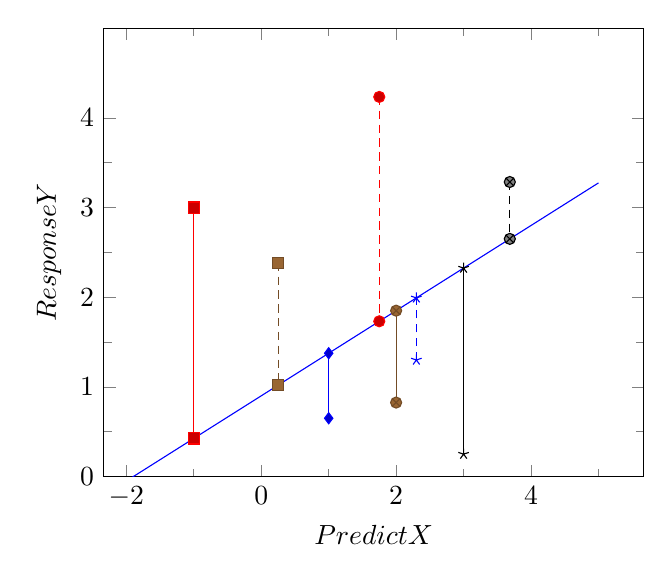
\begin{tikzpicture}
            \begin{axis}[
                xlabel=$Predict X$,		 
                ylabel={$Response Y$},
                minor x tick num={1}, 		
                minor y tick num={1},
                ymin = 0, ymax=5,		 
                ytick={0,1,2,3,4},
            ]
            \addplot[color=blue, mark=]{0.475*x + 0.9};
            \addplot coordinates {(-1,0.425) (-1,3)};
	        \addplot coordinates {(2,0.825) (2,1.85)};
	        \addplot coordinates {(3,0.25) (3,2.325)};
	        \addplot coordinates {(1,0.65) (1,1.375)};
	        \addplot coordinates {(1.75,4.234) (1.75,1.73125)};
	        \addplot coordinates {(0.25,2.385) (0.25,1.01875)};
	        \addplot coordinates {(3.685,3.285) (3.685,2.650375)};
	        \addplot coordinates {(2.3,1.3) (2.3,1.9925)};
            \end{axis}
        \end{tikzpicture}
        
        \textit{A schematic plot for ols fitting. Each data point is indicated by a small symbol. Points below the line have negative residuals, while points above the line have positive residuals.}
    \end{center}
    
    The criterion function for obtaining estimates is based on the residuals. The residuals reflect the inherent asymmetry in the roles of the response and the predictor in regression problems.
    
    The ols estimates are those values ${\beta_{0}}$ and ${\beta_{1}}$ that minimize the function. 
    
    \begin{align}
        RSS(\beta_{0}, \beta_{1}) = \displaystyle \sum _{i = 1} ^ {N}   |y_{i} - (\beta_{0} + \beta_{1} x_{i})| ^ 2
    \end{align}
    
    We call the quantity RSS${ \left (\hat{\beta}_{0},{\hat{\beta}_{1}} \right)}$ the \textit{residual sum of squares}, or just RSS.
    
    The least squares estimates can be derived in many ways, one of which is 
    
    \begin{align}
        \hat{\beta_{1}} = \dfrac{SXY}{SXX} = \dfrac
        {\displaystyle\sum(x_{i}-\overline{x})(y_{i}-\overline{y})}
        {\displaystyle \sum {\left(x_{i} - \overline{x}\right)}^2} 
        = r_{xy} \dfrac{SD_{x}}{SD_{y}}
        \\
        \hat{\beta_{0}} = \overline{y} - \hat{\beta_{1}} \overline{x}
    \end{align}
    The several forms for $\hat{\beta_{1}}$ are all equivalent.
    
    
    Using Forbes’ data, we will write $\overline{x}$ as the sample mean of \textit{Temp} and $\overline{y}$ as the sample mean of \textit{Lpres}. The quantities needed for computing the least squares estimators are: 
    
    \begin{center}
        \begin{tabular}{c c c}
            $\overline{x} = 202.95294118 $ & $SXX = 530.78235294 $ & $SXY = 475.31223529 $ \\
            $\overline{y} = 139.60529412 $ & $SYY = 427.79402353 $
        \end{tabular}
    \end{center}
    
    In case regression calculations are not done by using statistical software or a statistical calculator, intermediate calculations such as these should be done as accurately as possible, and rounding should only be used for final results. Using the above-mentioned results, we can find
    
    \begin{center}
        \begin{tabular}{c}
        ${\hat{\beta_{1}} = \dfrac{SXY}{SXX} = 0.895}$ \\
        ${\hat{\beta_{0}} = \overline{y} - \hat{\beta_{1}} \overline{x} = -42.138}$
        \end{tabular} 
    \end{center}
    
    The estimated line, given by both of the equations

    \begin{center}
        \begin{tabular}{c}
            ${\hat{E} (Lpres|Temp) = -42.138 + 0.895Temp}$ \\
        \end{tabular} 
    \end{center}

\section{Estimating $\sigma ^ {2}$}

    Although ${e}_{i}$ are not usually parameters, we will use the hat notation to specify the residuals: the residual for the $i^{th}$ case, denoted $\hat{e}_{i}$, is given by the equation
    
    \begin{align} 
        \hat{e _{i}} = \hat{y_{i}} - \hat\beta_{0} + \hat\beta_{1} 
    \end{align}
    
    which compares with the equation for the statistical errors
    
    \begin{align} 
        {e _{i}} = {y_{i}} - \beta_{0} + \beta_{1} 
    \end{align}
   
    For simple regression, residual $df$ $=$ $n - 2$ (with $n$ = 17, the number of data we are using; $df$ = number of cases minus the number of parameters in the mean function and $df$ is denoted from \textit{degrees of freedom}), so the estimate of $\sigma ^ 2$ is given by
    
    \begin{align} 
        {\sigma^2} = \dfrac{RSS}{n-2}
    \end{align}
    
    Using summaries from the given results ($\overline{x}, \overline{y}, ...$), we find
        
    \begin{center}
        \begin{tabular}{c c c}
            $RSS = SYY - \hat\beta_{1}^2 SXX = 2.15491$ \\
            $\sigma^2 = \dfrac{RSS}{n - 2} = 0.14366$
        \end{tabular}
    \end{center}
    
    The square root of $\sigma ^ 2$, $\sigma$ $=$ $\sqrt{0.14366}$ $=$ $0.37903$, is often called the standard error of regression. It's in the same units as is the response variable.
    
\section{Appendix A3} 
    The ols estimates of values ${\beta_{0}}$ and ${\beta_{1}}$ that minimize the function.
    
    \begin{align}
        RSS(\beta_{0}, \beta_{1}) = \displaystyle \sum _{i = 1} ^ {N}   |y_{i} - (\beta_{0} + \beta_{1} x_{i})| ^ 2
    \end{align}
    
    The method of finding the minimize is differentiate with respect to $\beta_{0}$ and $\beta_{1}$, and make it equal $0$. 
    
    \begin{align} 
        \dfrac{\partial RSS(\beta_{0}, \beta_{1}) }{\beta_{0}} = -2 \displaystyle \sum _{i=1}^{n}  (y_{i} - \beta_{0} - \beta_{1} x_{i}) = 0
        \\
        \dfrac{\partial RSS(\beta_{0}, \beta_{1}) }{\beta_{1}} = -2 \displaystyle \sum _{i=1}^{n}  x_{i} (y_{i} - \beta_{0} - \beta_{1} x_{i}) = 0
    \end{align}
        
    From (11), (12) we get (13) and (14) like this: 
    
    \begin{align} 
        \beta_{0} n + \beta_{1} \displaystyle \sum x_{i} = \displaystyle \sum y_{i}
        \\
        \beta_{0} \displaystyle \sum x_{i} + \beta_{1} \displaystyle \sum x_{i}^2 = \displaystyle \sum x_{i} y_{i}
    \end{align}
    
    Using fomulars: 
    
     \begin{align} 
        SXX &= \Sigma (x_{i} - \overline{x})^2 \\
        &= \Sigma x_{i}^2 - 2 \Sigma x_{i} \overline{x} + n\overline{x}^2  \nonumber \\
        &= \Sigma x_{i}^2 - 2 \Sigma x_{i} \dfrac{\Sigma x_{i}}{n} + n\dfrac{\Sigma x_{i} \Sigma x_{i}}{n^2}   \nonumber \\
        &= \Sigma x_{i}^2 - \dfrac{\Sigma x_{i} \Sigma x_{i}}{n} \nonumber \\
        &= \Sigma x_{i}^2 - n\dfrac{\Sigma x_{i} \Sigma x_{i}}{n n} \nonumber \\
        &= \Sigma x_{i}^2 - n\overline{x}^2 \nonumber \\
        SXY &= \Sigma (x_{i} - \overline{x})(y_{i} - \overline{y}) = \Sigma x_{i}y_{i} - n\overline{x}\overline{y}
    \end{align}
    
    Solving (13), (14), we get:
    
    \begin{align} 
        \beta_{0} &n + \beta_{1} \Sigma x_{i} = \Sigma y_{i}                \nonumber \\
        \beta_{0} &= \dfrac {\Sigma y}{n} - \beta_{1}  \dfrac {\Sigma x}{n} \nonumber \\
        \beta_{0} &= \overline{y} - \beta_{1}  \overline{x}                 \\
        \nonumber \\
        \nonumber \\
        \beta_{0} &\Sigma x_{i} + \beta_{1} \Sigma x_{i}^2 = \Sigma x_{i} y_{i} \nonumber \\
        \beta_{1} &= \dfrac{\Sigma x_{i}y_{i} - \beta _{0} \Sigma x_{i} }{ \Sigma x_{i}^2} \nonumber \\
        \beta_{1} &= \left ( \dfrac{\Sigma x_{i}y_{i}}{\Sigma x_{i}^2} - \dfrac{\Sigma x_{i} \Sigma y_{i}}{n \Sigma x_{i}^2} \right ) 
        \dfrac{n \Sigma x_{i}^2}{n\Sigma x_{i}^2 - \Sigma x_{i} \Sigma x_{i}} \nonumber \\
        \beta_{1} &= \left ( \Sigma x_{i}y_{i} - \dfrac{\Sigma x_{i} \Sigma y_{i}}{n} \right ) 
        \dfrac{n}{n\Sigma x_{i}^2 - \Sigma x_{i} \Sigma x_{i}} \nonumber \\
        \beta_{1} &= \dfrac{n \Sigma x_{i} y_{i} - \Sigma x_{i} \Sigma y_{i}}{n \Sigma x_{i}^2 - \Sigma x_{i} \Sigma x_{i}} \nonumber \\
        \beta_{1} &= \dfrac{\Sigma x_{i} y_{i} - n \overline{x} \overline{y}}{n \Sigma x_{i}^2 - n \overline{x}^2} \nonumber \\
        \beta_{1} &= \dfrac{SXY}{SXX}
    \end{align}
    
\section {About Forbes' Data}
    
    In an 1857 article, a Scottish physicist named James D. Forbes discussed a series of experiments that he had done concerning the relationship between atmospheric pressure and the boiling point of water. Forbes knew that the altitude could be determined from atmospheric pressure, measured with a barometer, with lower pressures corresponding to higher altitudes.
    
    In the middle of the nineteenth century, barometers were fragile instruments, so Forbes wondered if a simpler measurement of the boiling point of water could work as a substitute for a direct reading of barometric pressure. He collected data from 17 locations in the Alps and Scotland. He measured each location pressure in inches of mercury with a barometer and boiling point in degrees Fahrenheit. Let’s take a look at the scatter plot. Here is the scatter plot. % WTF man? %
    Of course we have to load the data first. After plotting the data, we add the best-fitting OLS line to the plot. This is the straight line that best fits the data according to the Ordinary Least Squares criterion, which we shall discuss in detail later.
    
\section {Linear Regression's Estimation Methods}
    
    These are some of the most common estimations for linear regression: 

    Least-squares estimation.
    
    Maximum-likelihood estimation.
    
    Bayesian linear regression.
    
    Quantile regression.
    
    Mixed models.
    
    Principal component regression.
    
    Least-angle regression.
    
    Theil–Sen estimator.
    
    \vspace{\baselineskip}
    
\section {References}
    \textit{James H. Steiger - Department of Psychology and Human Development Vanderbilt University}
%   
%\section{Further reading on} 
%    \textit{https://en.wikipedia.org/wiki/Simple_linear_regression}
%    
%    \textit{https://en.wikipedia.org/wiki/Linear_regression}
%    
\end{document}
